\section{Gradient-based design}\label{sec:gradient}

All operating points so far come from random search. The simulator is differentiable (Section~\ref{sec:lle}), so the device
parameters and the mask can also be treated as trainable and optimised along the gradient of the task error. A differentiable LLE
has been used to inverse-design comb spectra~\cite{chuchalin2026}; here the objective is the error of a computing task, with noise
inside the optimisation. This section tests whether this beats random search. In short, gradient fine-tuning reliably improves
its starting point, but ties with an enlarged random search that costs far less computation, so for our problem it cannot replace
random search and is at most a refinement after it.

\subsection{Training set-up}

The trainable quantities are the detuning, the input coupling $\Qone$, the pump power, the modulation depth and the complex biases
and weights of the 16 input lines (Eq.~\eqref{eq:mask}); the total optical input power is capped at the upper limit of the random
search. Each iteration runs several windows of the training series (400 symbols each, preceded by 100 gradient-free warm-up symbols),
each with several independent noise realisations, in one batch. A ridge readout is fitted in closed form on the first part of the
windows (pooled over windows and realisations), the NMSE is computed on the rest, and a consistency penalty is added (the variance of
the standardised features across noise realisations for the same input, close to 1 in the chaotic regime). The gradient flows through
the ridge regression, the readout and the whole LLE integration back to the device parameters. All realistic noise sources are on
during training and the readout must fit several noise realisations at once, so the optimisation targets the expected error over the
noise, and the readout cannot win by memorising one realisation.

Near the chaotic regime the loss landscape has cliffs: a small step across the border makes the comb non-reproducible and the
gradient diverges. We use four safeguards: gradients flow back through at most 16 symbols (truncated backpropagation through time);
gradient clipping; undoing any step after which the loss jumps far above its running average, then halving the learning rate; and a
cosine learning-rate decay. The parameters kept are those that score best on a separate validation series, and the reported error
comes from a third, test series.

\subsection{A grid-truncation trap}

Training uses a 256-mode spectral grid to save memory, and every result is re-simulated on 512 modes before it is reported. Early
training runs used 128 modes, which is too narrow for this device: training pushes the device towards broader spectra that fill the
whole grid. For example, a ring trained on 128 modes (no noise, Mackey--Glass) carries appreciable power in all 128 modes after
training; on a re-check with 256 modes and half the time step its spectrum spreads over 215 lines and the test error changes from
$8.5\times10^{-3}$ to $9.6\times10^{-3}$, about 14\%, more than the grid dependence of any other result in this paper
(Appendix~\ref{app:checks}). The truncation at the grid edge becomes a ``degree of freedom'' the optimiser can exploit, and part of
the resulting performance is an artefact of the discretisation. Design with a differentiable physical model therefore needs a grid
wide enough that truncation does not matter, and every trained result must be re-checked on a finer grid; all results in
Fig.~\ref{fig:gradient} were re-checked on 512 modes.

\subsection{Comparison with random search}

For a fair comparison we start from the same random operating points (realistic noise, 8-tap readout, Mackey--Glass, three series):
32 random points are ranked by validation error on the first series; the best four are fine-tuned with two training seeds each and
four points from the middle of the ranking once each, twelve runs of 60 steps in total. As a control, random search is extended from
32 to 256 points. All results are re-simulated on 512 modes with new noise realisations (Fig.~\ref{fig:gradient}).

\begin{figure}[htbp]
\centering
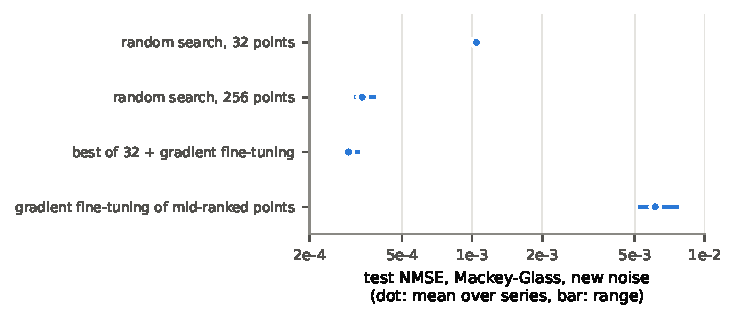
\includegraphics{fig7_gradient}
\caption{Gradient fine-tuning against random search (Mackey--Glass under realistic noise, 512 modes, new noise; dots are means over
three series, bars the range; a range smaller than the marker is hidden). Fine-tuning the best of 32 random points matches extending the random search to 256 points;
fine-tuning points from the middle of the ranking stays far behind the search.}
\label{fig:gradient}
\end{figure}

All twelve fine-tuning runs end better than their starting points, at 0.24 to 0.93 times the starting error, about 0.46 times on
geometric average. The best of 32 random points has $1.04\times10^{-3}$; fine-tuning from it reaches at best $2.9\times10^{-4}$;
extending random search to 256 points directly gives $3.4\times10^{-4}$. The two are comparable, within the spread between noise
realisations. Three further observations limit the role of fine-tuning: the same start with another training seed differs by almost a
factor of two ($2.9\times10^{-4}$ against $5.4\times10^{-4}$); starting from the middle of the ranking, fine-tuning stays above
$6\times10^{-3}$, far worse than the search, so it cannot rescue a mediocre start; and three of the twelve runs were still at their
best at the last validation (step 60), so these had not converged and longer training might help.
In computation random search wins clearly: on the same GPU each fine-tuning run (256 modes, 60 steps) takes about 18~s per step,
about 18 minutes per run and about 2.4 hours for the eight runs from the best four starts, whereas extending random search from 32 to
256 points adds one batched simulation per series (up to 512 operating points per batch, one to two minutes).

At the size of our problem (about 70 real parameters) random search alone is therefore the better choice; gradient fine-tuning is at
most a refinement after the search, and should be run with several training seeds. Differentiable simulation may be more valuable in
two situations: many more tunable quantities (a 64-line mask, or several rings designed together), where random search degrades
quickly while the cost of a gradient barely grows; and objectives with continuous structure that random sampling covers poorly.
Neither was tested here.
